\newpage
\section{Systemöversikt}
QuadOpt är uppdelat i flera mindre delsystem, för att vara mer lätthanterligt och lättare att utveckla.

\subsection{Systembeskrivning}
%QuadOpt kommer kunna köras via två olika typer av gränssnitt. Det ena är vårt egetutvecklade GUI och det andra är anrop via Matlab.

%\subsubsection{GUI}
%\subsubsection{Matlab}

Användaren har möjligheten att använda QuadOpt antingen via MATLAB eller via gruppens egna GUI. Om MATLAB används kommer den inskickade datan att konverteras till datastrukturer som kan läsas av QuadOpt via en specialfunktion skriven med MEX som förklaras mer exakt i avsnitt 4.2. Skulle istället GUI:t att användas, så kommer datan att konverteras som den står i gränssnittet med hjälp av en parser, som konverterar datan till en C-fil som man läsas direkt av QuadOpt innehållande alla datastrukturer som behövs, även detta beskrivs senare i avsnitt 4.5. Hur själva lösaren fungerar och löser problemet beskrivs i avsnitt 4.1 och matrisbiblioteket som den använder som innehåller de optimerade matrisoperatorer som behövs beskrivs i avsnitt 4.3.

\begin{figure}[h]
	\begin{center}
		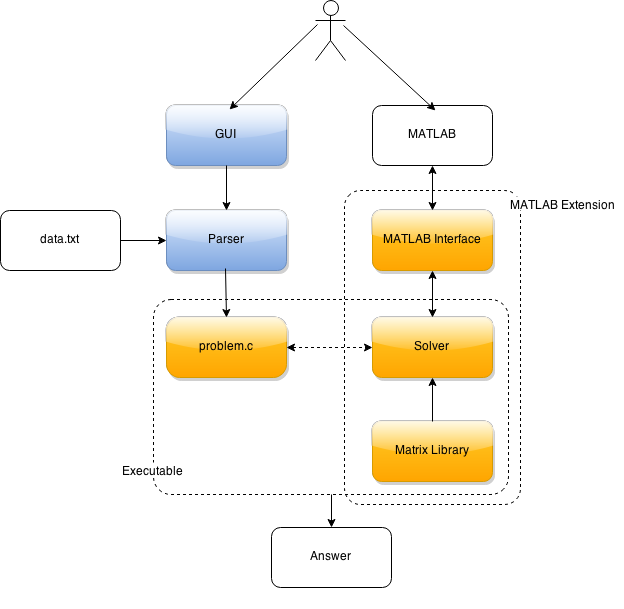
\includegraphics[scale=0.5]{bilder/arkitektur.png}
	\end{center}
	\caption{Arkitektur av systemet.}
\end{figure}

%\subsection{Beräkningar}
%Kommer utföras i lösaren, kommer använda vårt egna matrisbibliotek Matlib för att snabba upp beräkningarna.